\chapter{Results and evaluation}
\label{ch:results}

\section{Overview}

The next section describes the method used to gather data on the effectiveness of the learning ghost controller, with the results being presented in Section \ref{sec:results}.  Section \ref{sec:overfitting} investigates the problem of overfitting, and the final section explores possible improvements to the base MCTS algorithm.

\section{Method}

The learning ghost controller described in Chapter \ref{ch:design} was successfully implemented in Java using the IntelliJ development environment, and a server to facilitate testing the project, detailed in Chapter \ref{ch:verification}, was developed.  The server makes it possible to specify a set of parameters for the algorithm in a JavaScript file, and allows any number of connected machines to run the games specified by the scripts and report back the final scores.

A number of these parameter scripts were created to investigate various aspects of the algorithm, and these will be detailed below.  Due to the high variance in the final scores for a given parameter set, 20 games were run for each script and an average was obtained for each set.  Reference will be made to whether results are ``statistically significant'': a result is taken to be significantly different from another if a Student's t-test on the two data sets gives $p < 0.05$.

The games were run over 12 identical computers each with 3.3~GHz Intel i5 processors and 4~Gb of memory.  Since the computers have four cores, each computer ran two instances of the experiment client: this meant each computer could run two games at once, halving the amount of time needed whilst saving resources and electricity.  The cluster ran up to 24 games simultaneously, and around 2000 games were run over a few days; this would have taken 1--2 weeks without the experiment server.

\section{Results}
\label{sec:results}

\subsection{Learning vs non-learning controller}

The first experiment aimed to assess broadly whether the learning ghost controller improved performance.  It was initially assumed that the agent would have poor performance if the learning controller started off with zero knowledge, so it was supplied with weights trained from data recorded in a game against the {\tt Legacy} controller.  Figure \ref{fig:results1} shows the average final scores obtained after playing 20 games using each of the six sample ghost controllers as opponents, first using {\tt Legacy} during playouts as a ``non-learning'' controller, and again using the learning controller.

\begin{figure}
\centering
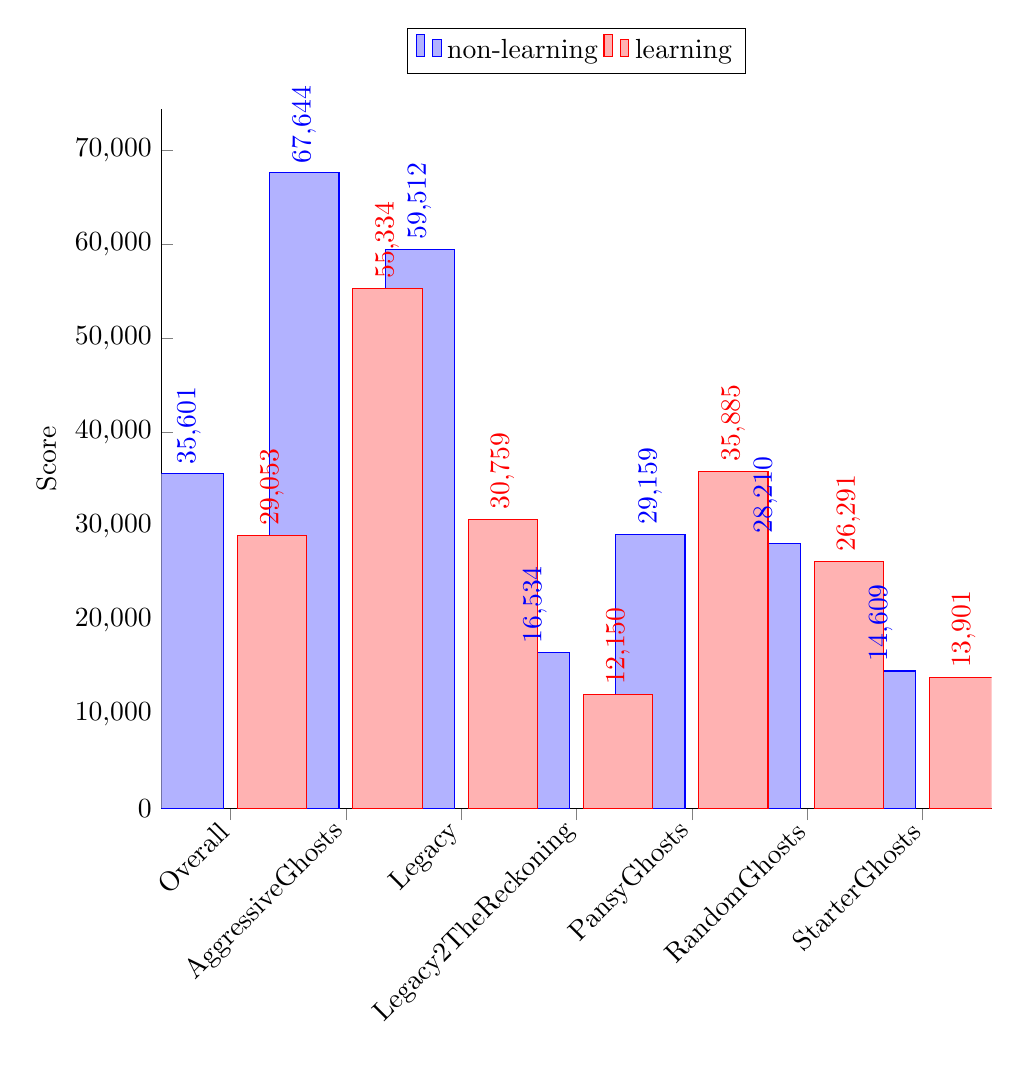
\begin{tikzpicture}
\pgfplotsset{every axis legend/.append style={
at={(0.5,1.05)},
anchor=south}}
\begin{axis}[
    %symbolic x coords={non-learning, learning},
    ybar = 5pt,
    symbolic x coords={Overall, AggressiveGhosts, Legacy, Legacy2TheReckoning, PansyGhosts, RandomGhosts, StarterGhosts},
    ylabel=Score,
    xtick=data,
    ymin=0,
    nodes near coords=\rotatebox{90}{\pgfmathprintnumber\pgfplotspointmeta},
    scaled y ticks=false,
    axis lines*=left,
    bar width=25pt,
    enlarge x limits=0.1,
    legend columns=4,
    width=\textwidth,
    x tick label style={rotate=45, anchor=east}
    ]
    
    \addplot coordinates {
       (Overall,35601)
       (AggressiveGhosts,67644)
       (Legacy,59512)
       (Legacy2TheReckoning,16534)
       (PansyGhosts,29159)
       (RandomGhosts,28210)
       (StarterGhosts,14609)
    };
    \addlegendentry{non-learning}
    
    \addplot coordinates {
       (Overall,29053)
       (AggressiveGhosts,55334)
       (Legacy,30759)
       (Legacy2TheReckoning,12150)
       (PansyGhosts,35885)
       (RandomGhosts,26291)
       (StarterGhosts,13901)
    };
    \addlegendentry{learning}
    
    
\end{axis}
\end{tikzpicture}
\caption[Learning vs non-learning ({\tt Legacy}) ghost controller]{Learning vs non-learning ({\tt Legacy}) ghost controller: averaged over all sample opponents, there is a decrease in performance when using the learning controller, but taking the {\tt PansyGhosts} controller on its own reveals an increase in performance.  Both results are statistically significant ($p < 0.05$).}
\label{fig:results1}
\end{figure}

\begin{figure}
\centering
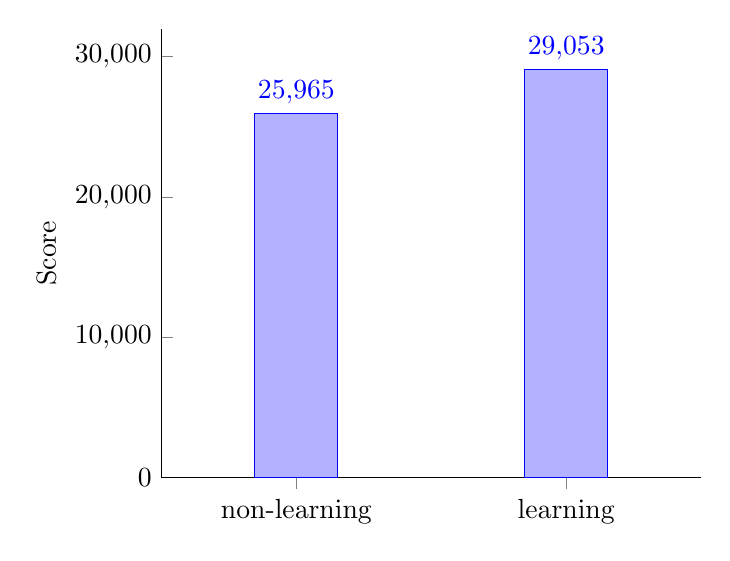
\begin{tikzpicture}
\pgfplotsset{every axis legend/.append style={
at={(0.5,-0.2)},
anchor=north}}
\begin{axis}[
    symbolic x coords={non-learning,learning},
    ylabel=Score,
    ybar=5pt,
    xtick=data,
    ymin=0,
    nodes near coords,
    scaled y ticks=false,
    axis lines*=left,
    bar width=30pt,
    enlarge x limits=0.5
    ]
    \addplot coordinates {
       (non-learning,25965)
       (learning,29053)
    };
\end{axis}
\end{tikzpicture}
\caption[Learning vs non-learning ({\tt RandomGhosts}) ghost controller]{Learning vs non-learning ({\tt RandomGhosts}) ghost controller: using the learning controller during rollouts shows slightly improved performance over using a random player, but not significantly so.}
\label{fig:resultsrandom}
\end{figure}

The results look at first glance disappointing, with the average over all 6 opponents being significantly lower when using the learning controller during playouts compared to using {\tt Legacy}; however, further investigation of the data revealed that performance against the {\tt PansyGhosts} controller showed a significant increase in performance as a result of using the learning controller.  Recall from Section \ref{sec:sampleghosts} that the {\tt PansyGhosts} controller causes all of the ghosts to always run away from Ms~Pac-Man, whilst the {\tt Legacy} controller causes three of the ghosts to always run towards Ms~Pac-Man: it would seem sensible that {\tt Legacy} would be a bad model for {\tt PansyGhosts} and thus the ability to learn the opposite behaviour of the opponent has clearly benefited the agent.  Figure \ref{fig:resultsrandom} shows that using the learning controller might be slightly better than using a random player, but the result is not statistically significant.

\subsection{Capping the rollout length}

It was conjectured that the reason for the lowered performance overall when using the learning controller is that time spent learning takes away from the time available to the MCTS algorithm, potentially leading to lower quality decisions.  Therefore the first experiment was repeated with the length of playouts (that is, the amount of \emph{game time} each playout is simulated for, not the length of time the simulation is run for) capped at 10 seconds, in the hope that the algorithm would be able to perform more playouts.  Figure \ref{fig:resultssr} shows that the learning controller still gives a decreased performance; in retrospect, the 10 second cap may still have been too high to really effect the outcome.

\begin{figure}
\centering
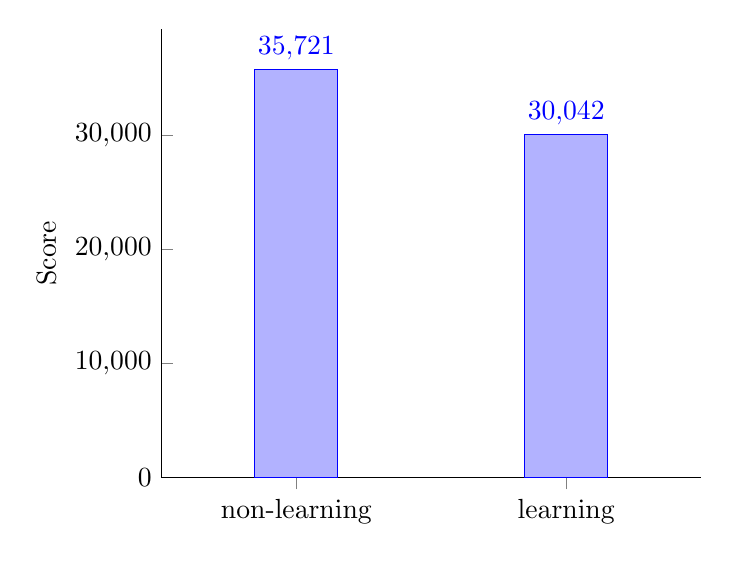
\begin{tikzpicture}
\pgfplotsset{every axis legend/.append style={
at={(0.5,-0.2)},
anchor=north}}
\begin{axis}[
    symbolic x coords={non-learning,learning},
    ylabel=Score,
    ybar=5pt,
    xtick=data,
    ymin=0,
    nodes near coords,
    scaled y ticks=false,
    axis lines*=left,
    bar width=30pt,
    enlarge x limits=0.5
    ]
    \addplot coordinates {
       (non-learning,35721)
       (learning,30042)
    };
\end{axis}
\end{tikzpicture}
\caption[Learning with a 10 second maximum rollout length]{Learning with a 10 second maximum rollout length: capping the rollout length at 10 seconds does not seem to alter the results much as they still show a decrease in performance when using the learning controller.}
\label{fig:resultssr}
\end{figure}

\subsection{Non-real-time learning}

In order to properly exclude the possibility that the time spent learning decreases the quality of the MCTS results, the first experiment was repeated; instead of running in real-time however, every decision was given exactly 1000 iterations of MCTS and the ghost neural networks were trained for exactly 100 iterations on every ghost decision observed.  The results in Figure \ref{fig:resultsrealtime} still show a decrease in overall performance when using the learning controller during playouts, but it is not a statistically significant difference.  The {\tt PansyGhosts} controller still shows a significant increase in performance.  It is not clear why the learning controller should not be at least as good as using {\tt Legacy} during playouts when the number of iterations of MCTS is fixed.

\begin{figure}
\centering
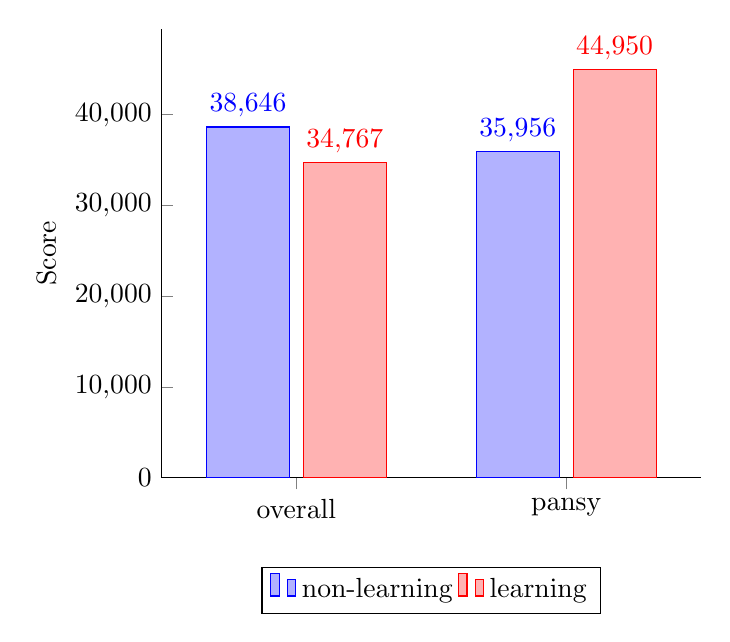
\begin{tikzpicture}
\pgfplotsset{every axis legend/.append style={
at={(0.5,-0.2)},
anchor=north}}
\begin{axis}[
    symbolic x coords={overall,pansy},
    ylabel=Score,
    ybar=5pt,
    xtick=data,
    ymin=0,
    nodes near coords,
    scaled y ticks=false,
    axis lines*=left,
    bar width=30pt,
    enlarge x limits=0.5,
    legend columns=4
    ]
    \addplot coordinates {
       (overall,38646)
       (pansy,35956)
    };
    \addlegendentry{non-learning}
    
    \addplot coordinates {
       (overall,34767)
       (pansy,44950)
    };
    \addlegendentry{learning}
\end{axis}
\end{tikzpicture}
\caption[Non-realtime learning]{Non-realtime learning: when every decision is given exactly 1000 iterations of MCTS and the ghost networks are trained exactly 100 times for every new example, the learning controller still fares slightly worse overall, but the result is not statistically significant.  On the other hand, {\tt PansyGhosts} taken on its own shows a statistically significant improvement with learning.}
\label{fig:resultsrealtime}
\end{figure}


\subsection{The effect of seeding the neural network}

The experiments described so far have used the learning controller initiated with weights trained from data recorded in a game against {\tt Legacy} (i.e., the controller should start off behaving like {\tt Legacy}).  This is because it was initially assumed that the agent would do really poorly to start off with until the ghost controller learned some behaviour, and that it may never get the chance to learn behaviour if the agent died early on as a result of poor decisions.  It was decided to verify this belief, and so 20 games were run against all 6 opponent controllers for each of the following four cases: real-time with and without pre-trained weights, and non-real-time with and without pre-trained weights.  The results are shown in Figure \ref{fig:resultsuntrained}, and they are somewhat surprising: using pre-trained weights confers no advantage.  It is conjectured that the ghost behaviour is actually rather easy to learn, and that it does not take long for this to happen.

\begin{figure}
\centering
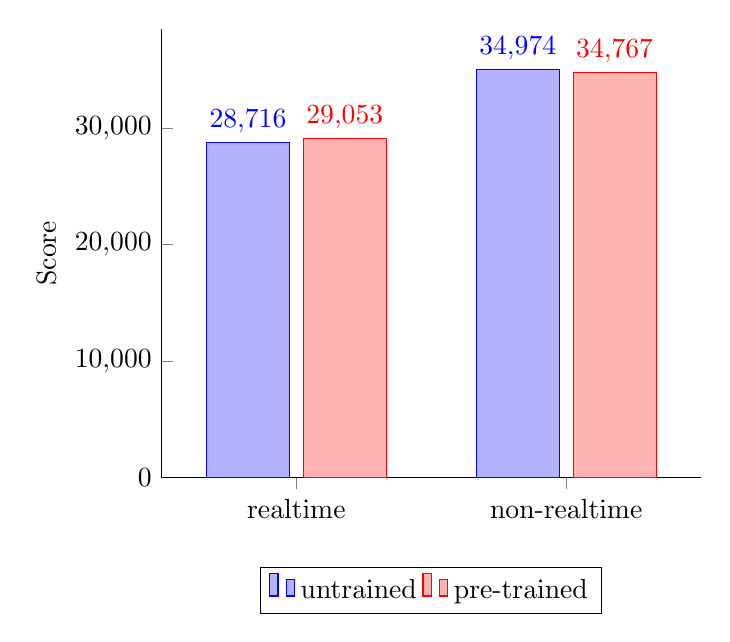
\begin{tikzpicture}
\pgfplotsset{every axis legend/.append style={
at={(0.5,-0.2)},
anchor=north}}
\begin{axis}[
    symbolic x coords={realtime,non-realtime},
    ylabel=Score,
    ybar=5pt,
    xtick=data,
    ymin=0,
    nodes near coords,
    scaled y ticks=false,
    axis lines*=left,
    bar width=30pt,
    enlarge x limits=0.5,
    legend columns=4
    ]
    \addplot coordinates {
       (realtime,28716)
       (non-realtime,34974)
    };
    \addlegendentry{untrained}
    
    \addplot coordinates {
       (realtime,29053)
       (non-realtime,34767)
    };
    \addlegendentry{pre-trained}
\end{axis}
\end{tikzpicture}
\caption[Untrained vs pretrained]{Untrained vs pretrained: supplying the learning controller with weights trained from {\tt Legacy} to start from confers no significant advantage, either in realtime or not.}
\label{fig:resultsuntrained}
\end{figure}


\subsection{The effect of varying the number of training iterations}

\begin{figure}
\centering
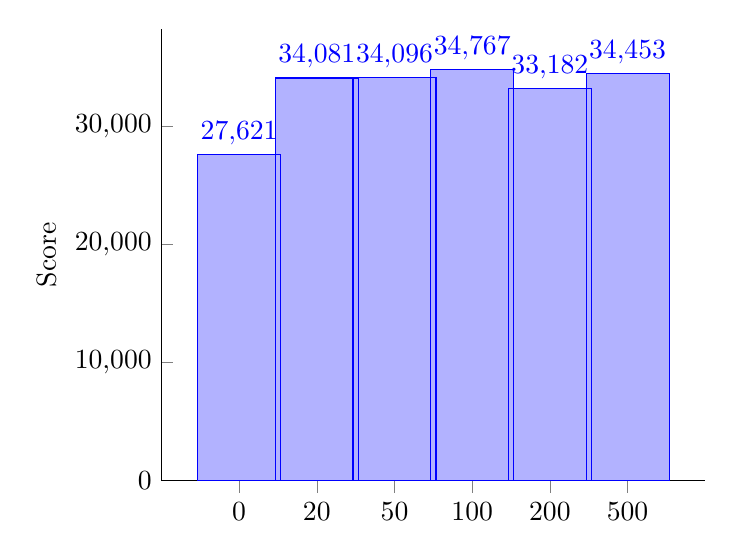
\begin{tikzpicture}
\pgfplotsset{every axis legend/.append style={
at={(0.5,-0.2)},
anchor=north}}
\begin{axis}[
    symbolic x coords={0,20,50,100,200,500},
    ylabel=Score,
    ybar=40pt,
    xtick=data,
    ymin=0,
    nodes near coords,
    scaled y ticks=false,
    axis lines*=left,
    bar width=30pt,
    enlarge x limits=0.2,
    width=0.7\textwidth
    ]
    \addplot coordinates {
       (0,27621)
       (20,34081)
       (50,34096)
       (100,34767)
       (200,33182)
       (500,34453)
    };
\end{axis}
\end{tikzpicture}
\caption[The effect of varying the number of training iterations]{The effect of varying the number of training iterations: there is no significant difference between any of the values, but 0 iterations gives noticeably lowered performance.}
\label{fig:resultsiterations}
\end{figure}


A series of experiments were run in non-real-time mode to investigate the effect of changing the number of iterations each new observed training example was learned over.  20 games were played against each of the 6 opponents, for each of the following iteration counts: 0, 20, 50, 100, 200 and 500.  In all cases except the first, the number of iterations of MCTS run was 1000.  Figure \ref{fig:resultsiterations} shows the results: varying the number of iterations of training does not alter the average final score achieved.  This lends further evidence to the conjecture that the ghost behaviour is particularly trivial for the network to learn, but shows that something is being learned at the start.


\subsection{The effect of move selection strategy}

\begin{figure}
\centering
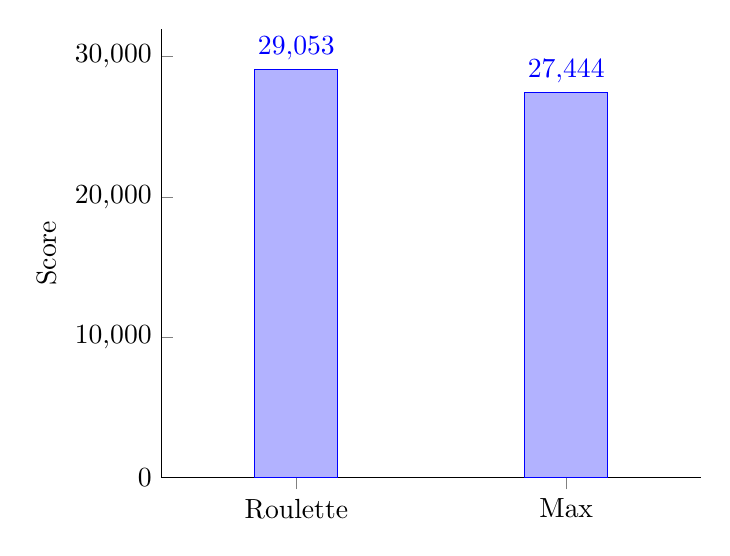
\begin{tikzpicture}
\pgfplotsset{every axis legend/.append style={
at={(0.5,-0.2)},
anchor=north}}
\begin{axis}[
    symbolic x coords={Roulette, Max},
    ylabel=Score,
    ybar=35pt,
    xtick=data,
    ymin=0,
    nodes near coords,
    scaled y ticks=false,
    axis lines*=left,
    bar width=30pt,
    enlarge x limits=0.5,
    ]
    \addplot coordinates {
       (Roulette,29053)
       (Max,27444)
    };
\end{axis}
\end{tikzpicture}
\caption[Roulette vs maximum move selection]{Roulette vs maximum move selection: using roulette selection is mariginally better than using maximum, but the result is not statistically significant.}
\label{fig:resultsmax}
\end{figure}

A final experiment was run to investigate the effect of the move selection strategy.  Recall from Section \ref{sec:nnalgorithm} the two ways of selecting a move from the neural network output: all the experiments described so far have used the {\tt RouletteSelectionStrategy} class, which selects a move with a probability proportional to its respective output.  This seems like a good strategy since Monte Carlo tree search is a probabilistic algorithm, and it would presumably help the performance if even unlikely game states are explored from time to time in case they are realised.  This hypothesis was verified by running 20 games using the learning controller in playouts against each of the 6 ghost teams, once using roulette selection and once using maximum selection.  The results are shown in Figure \ref{fig:resultsmax}: roulette selection does indeed appear to be slightly better than maximum selection, but again the result is not statistically significant.

\subsection{Statistical significance}

Lastly, a note on statistical significance.  Many of the results presented here are not statistically significant---the final scores obtained from the game for each experiment run have a high level of variance, as subtly different choices in each game can result in drastic differences in score, making it difficult to draw strong conclusions.  This could be ameliorated by running substantially more games, as 20 may not have been enough due to the high variance, but the time constraints of the project limited the total number of games that could be run.

\section{The problem of overfitting}
\label{sec:overfitting}

Overfitting is a problem where a learning algorithm can classify the training set really well, but is unable to generalise well.  The neural networks in the project were verified against the same data as they were trained with---it was realised towards the end of the project that this could be a source of error in the reported results, so it was decided to investigate the issue.  Two games were recorded for every ghost team and in the first case, the neural networks were trained and verified with the same data; in the second, they were trained with data from one game and verified with the data from the other recorded game.  By verified, it is meant that the neural network was allowed to make a prediction for each of the rows of data, and the prediction was checked against the actual output; the number of wrong predictions out of the total number of rows of data gives an error percentage.

The results are shown in Figure \ref{fig:resultsclasserror}: the reported error is much higher when a diffent data set is used for verification, so overfitting is an issue.  There are various ways to mitigate this, such as training on more examples, or using a better algorithm more immune to overfitting.  It could also be that the inputs to the neural network were poorly chosen.  For example, rather than feeding the next direction towards and away from Ms~Pac-Man as inputs and outputting a direction, the network could instead output a value which makes the choice to go towards or away.

Another interesting result shown in the graph is that the {\tt PansyGhosts} controller has a very low error, but it is not clear why this is the case.  It is a completely deterministic model, but so is {\tt AggressiveGhosts} for example, which has a much higher error.  It may have to do with the fact that two different distance measurements are used for chasing Pac-Man, and only one for running away, but more investigation is clearly warranted into this result.

\begin{figure}
\centering
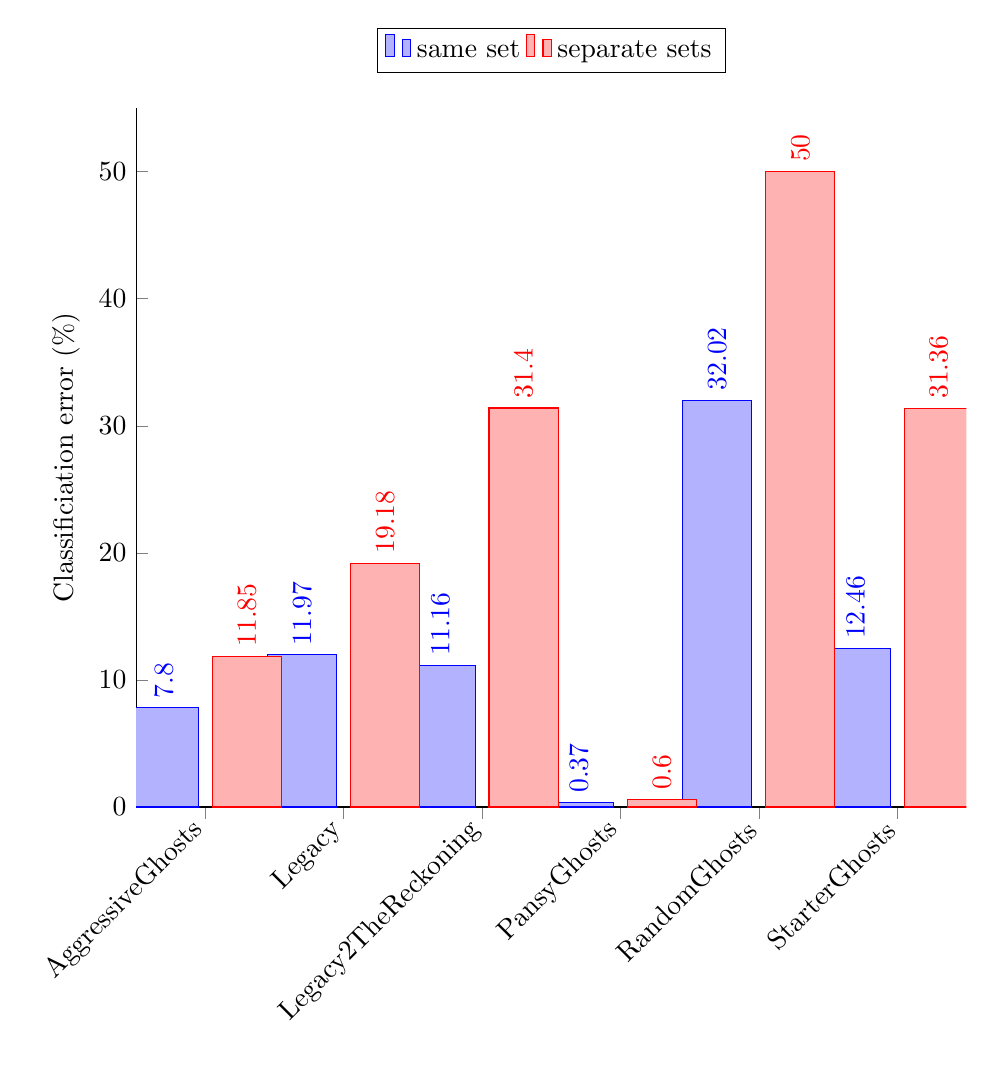
\begin{tikzpicture}
\pgfplotsset{every axis legend/.append style={
at={(0.5,1.05)},
anchor=south}}
\begin{axis}[
    ybar=5pt,
    symbolic x coords={AggressiveGhosts, Legacy, Legacy2TheReckoning, PansyGhosts, RandomGhosts, StarterGhosts},
    ylabel=Classificiation error (\%),
    xtick=data,
    ymin=0,
    nodes near coords=\rotatebox{90}{\pgfmathprintnumber\pgfplotspointmeta},
    scaled y ticks=false,
    axis lines*=left,
    bar width=25pt,
    enlarge x limits=0.1,
    legend columns=4,
    width=\textwidth,
    x tick label style={rotate=45, anchor=east}
    ]
    
    \addplot coordinates {
        (AggressiveGhosts,7.80)
        (Legacy,11.97)
        (Legacy2TheReckoning,11.16)
        (PansyGhosts,0.37)
        (RandomGhosts,32.02)
        (StarterGhosts,12.46)
    };
    \addlegendentry{same set}
    
    \addplot coordinates {
        (AggressiveGhosts,11.85)
        (Legacy,19.18)
        (Legacy2TheReckoning,31.4)
        (PansyGhosts,0.6)
        (RandomGhosts,50)
        (StarterGhosts,31.36)
    };
    \addlegendentry{separate sets}
\end{axis}
\end{tikzpicture}
\caption[Classification error when learning different ghost models]{Classification error when learning different ghost models: the error is shown for two cases, the first where the same set was used for training and verification, and the second where two different sets were used for training and validation in each case.}
\label{fig:resultsclasserror}
\end{figure}


\section{Ideas for improving the base MCTS algorithm}
\label{sec:maastricht}

The current best plain MCTS agents are better than the agent used in this project, achieving significantly higher scores.  A particularly good example is the ``maastricht'' agent developed by \citep{Pepels2012}.  This agent has various differences in its algorithms which may contribute to its greater success---it was intended to trial these potential improvements on the agent used in this project, but there was not enough time.  The differences are summarised here for reference and potential future work.

First of all, nodes represetning a reversal in direction for Ms~Pac-Man are not considered past the first layer on the tree.  The agent in this work can consider a potentially infinite sequence of reversals, taking up a lot of processing time and not contributing much knowledge to the tree.

Similar to the agent described by \cite{Ikehata2011}, the agent operates in one of three states: \emph{Ghost score}, \emph{Pill score}, and \emph{survival}. This enables the agent to change its behaviour depending on local conditions, such as whether or not a ghost is nearby.  The algorithm also encodes some long term goals to help bring the agent closer to scoring opportunities that can be missed by the MCTS algorithm.

If during the selection phase Ms~Pac-Man loses a life, the playout phase is re-started from the last visited junction.  If Ms~Pac-Man eats a ghost or power pill during the selction phase, the rollout is started immediately, as the ghost state is unpredictable.  The depth of the tree is limited to only include nodes a certain predefined distance from the agent's current location.  This may increase the space explored, and there is not much point simulating very far into the future due to the non-determinism of the ghosts.

The playouts during the simulation phase have different stopping conditions: their agent stops the playout if Ms~Pac-Man loses a life, a certain number of ticks have passed, the next level is reached, or Ms~Pac-Man eats a power pill while a previous power pill is active.  The latter is included to act as a punishment for making this poor choice.



